%*************************************************
% A template for MSc Thesis. 
% Please see "guideline.pdf" first.
%*************************************************
% Iman Izadi - Ehsan Karimi, 1400
% Dept. of Electrical and Computer Engineering, IUT
%*************************************************

\documentclass[a4paper,fleqn]{report} 

% All the packages and general definitions are included in this file: preamble.tex
%*************************************************
% All the packages and definitions required for this 
% project are included here.
%*************************************************
% This template is a modified version of the following template:
% Iman Izadi, 1395
% Dept. of Electrical and Computer Engineering, IUT
%*************************************************


\usepackage{amsthm,amssymb,amsmath}			% Writing math
\newcommand{\norm}[1]{\left\lVert#1\right\rVert}

\usepackage{cite} % added by Ehsan %https://tex.stackexchange.com/questions/29191/automatically-reorder-in-text-citations-based-on-numbering-in-bibliography

\usepackage{epsf,graphicx}					%Including graphics
\usepackage{subfig,graphicx} 


\usepackage[a4paper]{geometry}							% Fixing page layout and margins
\usepackage{titlesec}											% Change chapter and section titles
\usepackage{setspace}											% Change line spacing
\usepackage[stable,bottom]{footmisc}					% Move footnotes to the bottom of page
\usepackage{notoccite}
%\usepackage{enumitem}
\usepackage{enumerate}
\usepackage{comment}

\usepackage{zref-perpage}
\zmakeperpage[1]{footnote}
\usepackage{algorithm} %added by Ehsan for algorithms

\usepackage{enumitem}%added by Ehsan for bolding the title of items 
\newenvironment{descitemize} % a mixture of description and itemize
{\begin{description}[leftmargin=*,before=\let\makelabel\descitemlabel]}
	{\end{description}}

\newcommand{\descitemlabel}[1]{%
	\textbullet\ \textbf{#1}%
}


\usepackage[final]{showkeys} % added by Ehsan to show labels in pdf for easy referencing, 'final' to turn off all the package's functionality

\usepackage[obeyspaces,hyphens,spaces]{url}% added by ehsan
\renewcommand*{\showkeyslabelformat}[1]{%
	\fbox{\vbox{\hsize=1.1cm\normalfont\small\url{#1}\par}}}
%\usepackage[right]{showlabels} %final, margin,  right

\usepackage{indentfirst}			%tab befor each parapraph

\usepackage[hidelinks]{hyperref}				%added by ehsan to link ref number to refferences
\hypersetup{									% added by ehsan
%	bookmarks=true,         % show bookmarks bar?
	unicode=True,          % non-Latin characters in Acrobat’s bookmarks
	pdftoolbar=true,        % show Acrobat’s toolbar?
	pdfmenubar=true,        % show Acrobat’s menu?
	pdfauthor={Ehsan Karimi},     % author
	pdftitle = {Master Thesis },
	pdfkeywords={Dementia, 3D Deep Neural Network, Alzheimer Diseas Prediction}, 
	pdfcreator={Ehsan Karimi},
	colorlinks=true,       % false: boxed links; true: colored links
	linkcolor=blue,        % color of internal links (change box color with linkbordercolor)
	citecolor=blue,        % color of links to bibliography
	filecolor=blue,        % color of file links
	urlcolor=blue        % color of external links
}


\usepackage[flushleft]{threeparttable} %added by ehsan for table endnotes
\usepackage{rotating} %added by ehsan to rotate the table
\newcommand\myfrac[2]{\frac{#1}{#2\mathstrut}} %added by ehsan
\usepackage{makecell} %added by ehsan, to create a cell with multiple lines in tables

\usepackage{romannum} %added by ehsan for roman numbers
\usepackage[xindy,acronym,nonumberlist=true]{glossaries}	%added by ehsan for "vaje name" generation

\usepackage{xepersian}										% Persian , option "\KashidaOn" added by ehsan

\defpersianfont\nastaliq{IranNastaliq} %added by ehsan for thank U page

\settextfont{XB Zar}												% Persian font
%\setdigitfont{Yas}
\setcounter{tocdepth}{3}%added by ehsan to increas the levels in table of contents
%\setcounter{secnumdepth}{4}%added by ehsan to increas the levels in table of contents
%active glossaries
%\makeglossaries


%
\usepackage{multirow}
\usepackage{booktabs} %added by ehsan, its imported for table because https://www.latex-tables.com/


%added by ehsan to use a3page in the middel of document
\usepackage{lipsum}
\makeatletter
% like \newgeometry, but also allows change of landscape/portrait and paper size
% to be used with caution!
\newcommand{\newgeometryfull}[1]{%
	\clearpage
	\Gm@restore@org
	\Gm@initnewgm
	%  \Gm@newgmtrue
	\setkeys{Gm}{#1}%
	%  \Gm@newgmfalse
	\Gm@process
	\ifnum\mag=\@m\else\Gm@magtooffset\fi
	\Gm@changelayout
	\Gm@showparams{newgeometry}}%
\makeatother

%% Allow A3 sheets - - New environment
\newenvironment{a3page}{%
	\newgeometryfull{a3paper,landscape,width=360 mm,top=25 mm,bottom=25 mm}
	% set the correct dimension for the PDF viewer
	\pdfpageheight=\paperheight
	\pdfpagewidth=\paperwidth
}{%
	\restoregeometry
	% set the correct dimension for the PDF viewer
	\pdfpageheight=\paperheight
	\pdfpagewidth=\paperwidth
}







% Use English digits in equations
\DefaultMathsDigits

% Default footnotes from left to right
\setfootnoteLR

% Use English numbers for English footnotes
\makeatletter
\def\@makeLTRfnmark{\hbox{\@textsuperscript{\latinfont\@thefnmark}}}
\renewcommand\@makefntext[1]{%
    \parindent 1em%
    \noindent
    \hb@xt@1.8em{\hss\if@RTL\@makefnmark\else\@makeLTRfnmark\fi}#1}
\makeatother

% Use dash instead of dot in section numbers
\SepMark{-}										


% Change fonts and margins of section and subsection titles
% For chapters please see firstpages.tex
\titlespacing*{\section}{0pt}{1cm}{0.2cm}
\titleformat{\section}
  {\fontsize{12}{6}\scshape\bfseries}{\thesection}{1em}{}

\titlespacing*{\subsection}{0pt}{.8cm}{0cm}
\titleformat{\subsection}
  {\fontsize{11}{6}\scshape\bfseries}{\thesubsection}{1em}{}
  

\setcounter{secnumdepth}{3}

\titleformat{\paragraph}
{\normalfont\normalsize\bfseries}{\theparagraph}{1em}{}
\titlespacing*{\paragraph}
{0pt}{3.25ex plus 1ex minus .2ex}{1.5ex plus .2ex}

  
% Fix table of contents for chapters
\makeatletter 
\def\@chapter[#1]#2{\ifnum \c@secnumdepth >\m@ne
     \refstepcounter{chapter}%
     \typeout{\@chapapp\space\thechapter.}%
     \addcontentsline{toc}{chapter}%
       	{\@chapapp~\protect\numberline{\tartibi{chapter}\,:\space #1}}
  \else
  	 \addcontentsline{toc}{chapter}{#1}%
  \fi
  \chaptermark{#1}%
  \addtocontents{lof}{\protect\addvspace{10\p@}}%
  \addtocontents{lot}{\protect\addvspace{10\p@}}%
  \@makechapterhead{#2}%
  \@afterheading}
  \let\stdl@chapter\l@chapter
 \renewcommand*{\l@chapter}[2]{\stdl@chapter{{#1}}{}}
\makeatother

%%%%%%%%%%%%%%%%%%%%%%%%% my changes %%%%%%%%%%%%%%%%

%%%%%%%%%%%%%%%%%%%%%%%%%%%%%%%%%%%%%%%%%%%%%%%%%%%%%							

%set precompile dictionary settings
%اعمال تنظیمات واژه نامه fa-en، en-fa و لیست اختصارات
%%%%%%%%%%%%%%%%%%%%
%% تعریف استایل برای واژه نامه فارسی به انگلیسی،%%%%%% ============================================================================================================

%%% تنظیمات مربوط به بسته  glossaries
%%% تعریف استایل برای واژه نامه فارسی به انگلیسی، در این استایل واژه‌های فارسی در سمت راست و واژه‌های انگلیسی در سمت چپ خواهند آمد. از حالت گروه ‌بندی استفاده می‌کنیم، 
%%% یعنی واژه‌ها در گروه‌هایی به ترتیب حروف الفبا مرتب می‌شوند، مثلا:
%%% الف
%%% اقتصاد ................................... Economy
%%% اشکال ........................................ Failure
%%% ش
%%% شبکه ...................................... Network
\newglossarystyle{myFaToEn}{%
	\renewenvironment{theglossary}{}{}
	\renewcommand*{\glsgroupskip}{\vskip 10mm}
	\renewcommand*{\glsgroupheading}[1]{\subsection*{\glsgetgrouptitle{##1}}}
	\renewcommand*{\glossentry}[2]{\noindent\glsentryname{##1}\dotfill\space \glsentrytext{##1}
		
	}
}

%% % تعریف استایل برای واژه نامه انگلیسی به فارسی، در این استایل واژه‌های فارسی در سمت راست و واژه‌های انگلیسی در سمت چپ خواهند آمد. از حالت گروه ‌بندی استفاده می‌کنیم، 
%% % یعنی واژه‌ها در گروه‌هایی به ترتیب حروف الفبا مرتب می‌شوند، مثلا:
%% % E
%%% Economy ............................... اقتصاد
%% % F
%% % Failure................................... اشکال
%% %N
%% % Network ................................. شبکه

\newglossarystyle{myEntoFa}{%
	%%% این دستور در حقیقت عملیات گروه‌بندی را انجام می‌دهد. بدین صورت که واژه‌ها در بخش‌های جداگانه گروه‌بندی می‌شوند، 
	%%% عنوان بخش همان نام حرفی است که هر واژه در آن گروه با آن شروع شده است. 
	\renewenvironment{theglossary}{}{}
	\renewcommand*{\glsgroupskip}{\vskip 10mm}
	\renewcommand*{\glsgroupheading}[1]{\begin{LTR} \subsection*{\glsgetgrouptitle{##1}} \end{LTR}}
	%%% در این دستور نحوه نمایش واژه‌ها می‌آید. در این جا واژه فارسی در سمت راست و واژه انگلیسی در سمت چپ قرار داده شده است، و بین آن با نقطه پر می‌شود. 
	\renewcommand*{\glossentry}[2]{\noindent\glsentrytext{##1}\dotfill\space \glsentryname{##1}
		
	}
}

%%% تعیین استایل برای فهرست اختصارات
\newglossarystyle{myAbbrlist}{%
	%%% این دستور در حقیقت عملیات گروه‌بندی را انجام می‌دهد. بدین صورت که اختصارات‌ در بخش‌های جداگانه گروه‌بندی می‌شوند، 
	%%% عنوان بخش همان نام حرفی است که هر اختصار در آن گروه با آن شروع شده است. 
	\renewenvironment{theglossary}{}{}
	\renewcommand*{\glsgroupskip}{\vskip 7mm}
	\renewcommand*{\glsgroupheading}[1]{\begin{LTR} \subsection*{\glsgetgrouptitle{##1}} \end{LTR}}
	%%% در این دستور نحوه نمایش اختصارات می‌آید. در این جا حالت کوچک اختصار در سمت چپ و حالت بزرگ در سمت راست قرار داده شده است، و بین آن با نقطه پر می‌شود. 
	\renewcommand*{\glossentry}[2]{\noindent\glsentrytext{##1}\space\dotfill\space \Glsentrylong{##1}
		
	}
	%%% تغییر نام محیط abbreviation به فهرست اختصارات
	\renewcommand*{\acronymname}{\rl{فهرست اختصارات}}
}

%%% برای اجرا xindy بر روی فایل .tex و تولید واژه‌نامه‌ها و فهرست اختصارات و فهرست نمادها یکسری  فایل تعریف شده است.‌ Latex داده های مربوط به واژه نامه و .. را در این 
%%%  فایل‌ها نگهداری می‌کند. مهم‌ترین option‌ این قسمت این است که 
%%% عنوان واژه‌نامه‌ها و یا فهرست اختصارات و یا فهرست نمادها را می‌توانید در این‌جا مشخص کنید. 
%%% در این جا عباراتی مثل glg، gls، glo و ... پسوند فایل‌هایی است که برای xindy بکار می‌روند. 

\newglossary[blg]{persian}{bls}{blo}{واژه‌نامه فارسی به انگلیسی}
\newglossary[glg]{english}{gls}{glo}{واژه‌نامه انگلیسی به فارسی}
\makeglossaries
\glsdisablehyper
%%% تعاریف مربوط به تولید واژه نامه و فهرست اختصارات و فهرست نمادها
%%%  در این فایل یکسری دستورات عمومی برای وارد کردن واژه‌نامه آمده است.
%%%  به دلیل این‌که قرار است این دستورات پایه‌ای را بازنویسی کنیم در این‌جا تعریف می‌کنیم. 
\let\oldgls\gls
\let\oldglspl\glspl

\makeatletter

\renewrobustcmd*{\gls}{\@ifstar\@msgls\@mgls}
\newcommand*{\@mgls}[1] {\ifthenelse{\equal{\glsentrytype{#1}}{english}}{\oldgls{#1}\glsuseri{f-#1}}{\lr{\oldgls{#1}}}}
\newcommand*{\@msgls}[1]{\ifthenelse{\equal{\glsentrytype{#1}}{english}}{\glstext{#1}\glsuseri{f-#1}}{\lr{\glsentryname{#1}}}}

\renewrobustcmd*{\glspl}{\@ifstar\@msglspl\@mglspl}
\newcommand*{\@mglspl}[1] {\ifthenelse{\equal{\glsentrytype{#1}}{english}}{\oldglspl{#1}\glsuseri{f-#1}}{\oldglspl{#1}}}
\newcommand*{\@msglspl}[1]{\ifthenelse{\equal{\glsentrytype{#1}}{english}}{\glsplural{#1}\glsuseri{f-#1}}{\glsentryplural{#1}}}

\makeatother

\newcommand{\newword}[4]{
	\newglossaryentry{#1}     {type={english},name={\lr{#2}},plural={#4},text={#3},description={}}
	\newglossaryentry{f-#1} {type={persian},name={#3},text={\lr{#2}},description={}}
}

%%% بر طبق این دستور، در اولین باری که واژه مورد نظر از واژه‌نامه وارد شود، پاورقی زده می‌شود. 
\defglsentryfmt[english]{\glsgenentryfmt\ifglsused{\glslabel}{}{\LTRfootnote{\glsentryname{\glslabel}}}}

% این دستور اختصارات را علاوه بر فهرست اختصارات در پاورقی هم می‌آورد
%\defglsentryfmt[acronym]{\glsentryname{\glslabel}\ifglsused{\glslabel}{}{\LTRfootnote{\glsentrydesc{\glslabel}}}} % main (changed by ehsan)
%این دستور جایگزین دستور قبلی شده توسط ehsan و اختصارات را فقط در فهرست اختصارات می آورد و پاورقی نمیزند
\defglsentryfmt[acronym]{\glsentryname{\glslabel}\ifglsused{\glslabel}{}{}} % added by ehsan

%%%%%% ============================================================================================================

%%============================ دستور برای قرار دادن فهرست اختصارات 
\newcommand{\printabbreviation}{
	\cleardoublepage
	\phantomsection
	\baselineskip=.75cm
	%% با این دستور عنوان فهرست اختصارات به فهرست مطالب اضافه می‌شود. 
	%\addcontentsline{toc}{chapter}{فهرست اختصارات} % main (changed by ehsan)
	\addcontentsline{toc}{section}{فهرست اختصارات}  % added by ehsan
	\setglossarystyle{myAbbrlist}
	\begin{LTR}
		\Oldprintglossary[type=acronym]	
	\end{LTR}
	\clearpage
}%

\newcommand{\printacronyms}{\printabbreviation}
%%% در این جا محیط هر دو واژه نامه را باز تعریف کرده ایم، تا اولا مشکل قرار دادن صفحه اضافی را حل کنیم، ثانیا عنوان واژه نامه ها را با دستور addcontentlist وارد فهرست مطالب کرده ایم.
\let\Oldprintglossary\printglossary
\renewcommand{\printglossary}{
	\let\appendix\relax
	
	
%\begin{comment}
	%% تنظیم کننده فاصله بین خطوط در این قسمت
	\clearpage
	\phantomsection
	%% این دستور موجب این می‌شود که واژه‌نامه‌ها در  حالت دو ستونی نوشته شود. 
%	\twocolumn{}
	\onecolumn{}
	%% با این دستور عنوان واژه‌نامه به فهرست مطالب اضافه می‌شود. 
%	\addcontentsline{toc}{chapter}{واژه نامه انگلیسی به فارسی} % main (changed by ehsan)
	\addcontentsline{toc}{section}{واژه نامه انگلیسی به فارسی}  % added by ehsan
	\setglossarystyle{myEntoFa}
	\Oldprintglossary[type=english]
%	\end{comment}
	
	\clearpage
	\phantomsection
	%% با این دستور عنوان واژه‌نامه به فهرست مطالب اضافه می‌شود. 
%	\addcontentsline{toc}{chapter}{واژه نامه فارسی به انگلیسی} % main (changed by ehsan)
	\addcontentsline{toc}{section}{واژه نامه فارسی به انگلیسی}  % added by ehsan
	\setglossarystyle{myFaToEn}
	\Oldprintglossary[type=persian]
	\onecolumn{}
}%

%%%%%%

%read dictionary document 
%وارد کردن فهرست کلمات معادل و اختصار از فایل های دیکشنری

%this is derived by ehsan karimi
%see more: http://www.parsilatex.com/wiki/%D8%B1%D8%A7%D9%87%D9%86%D9%85%D8%A7%DB%8C_%D8%A7%DB%8C%D8%AC%D8%A7%D8%AF_%D9%88%D8%A7%DA%98%D9%87%E2%80%8C%D9%86%D8%A7%D9%85%D9%87
%_______________________________ ACN list ____________________________________

\newacronym{ML}{ML}{Machine Learning}
\newacronym{DL}{DL}{Deep Learning}
\newacronym{DBN}{DBN}{Deep Blief Network}
\newacronym{SVM}{SVM}{Support Vector Machine}
\newacronym{CNN}{CNN}{Convlutional Neural Network}
\newacronym{SGL}{SGL}{Sparse Group Lasso}
\newacronym{LSTM}{LSTM}{Long Short-Term Memory}

\newacronym{TP}{TP}{True Positives}
\newacronym{FP}{FP}{False Positives}
\newacronym{TN}{TN}{True Negetives}
\newacronym{FN}{FN}{False Negetives}

\newacronym{LASSO}{LASSO}{Least Absolute Shrinkage and Selection Operator}
\newacronym{RFP}{RFP}{Random Feature Projection}
\newacronym{CART}{CART}{Classification and Regression Trees}

\newacronym{VOI}{VOI}{Volume Of Interest}
\newacronym{GA}{GA}{Genetic Algorithm}
\newacronym{RFE}{RFE}{Recursive Feature Elimination}
\newacronym{GRU}{GRU}{Gated Recurrent Unit}
\newacronym{AE}{AE}{Autoencoder}


\newacronym{FDR}{FDR}{Fisher's Discriminant Ratio}


%_______________________________ Dict list ____________________________________
\newword{1st}{First}{اول}{اول‌ها}
\newword{2nd}{Second}{دوم}{دوم‌ها}
\newword{3rd}{Third}{سوم}{سوم‌ها}

%%%%%%%%%%%%%%%%

\newword{variance}{Variance}{واریانس}{}
\newword{bias}{Bias}{سوگیری}{}
\newword{dataset}{Data Set}{مجموعه داده}{مجموعه‌های داده}
\newword{noise}{Noise}{نویز}{}



%http://qa.parsilatex.com/16166/%D9%85%D8%B4%DA%A9%D9%84-%D8%AF%D8%B1-%D8%A7%DB%8C%D8%AC%D8%A7%D8%AF-%D9%88%D8%A7%DA%98%D9%87-%D9%86%D8%A7%D9%85%D9%87-%D8%A8%D8%A7-%D8%A7%D8%B3%D8%AA%D9%81%D8%A7%D8%AF%D9%87-%D8%A7%D8%B2-%D8%A8%D8%B3%D8%AA%D9%87-glossaries


\begin{document}

% The first pages (before abstract) are included in this file: firstpages.tex
%*************************************************
% In this file the first few pages are typeset.
% Make changes accordingly.
%*************************************************

% شماره صفحات با حروف
\pagenumbering{adadi}

%***************************
% Page 0: white paper
%***************************
\thispagestyle{empty}
\begin{center}
	~\vfill
%	
\includegraphics[scale=1]{images/besm.jpg}
	~\vfill
\end{center}
\pagebreak

%***************************
% Page 1: Besmelah
%***************************
\thispagestyle{empty}
\begin{center}
	~\vfill
	
\includegraphics[scale=1]{images/besm.jpg}
	~\vfill
\end{center}
\pagebreak

%***************************
% Page 2: Title
%***************************
\thispagestyle{empty}
\newgeometry{left=3cm,right=3cm,top=2cm}
\begin{center}

\includegraphics[height=3cm]{images/iut_logo.png}
\vspace{0.4cm}

{\large
	\textbf{دانشگاه صنعتی اصفهان}\\
	دانشکده مهندسی برق و کامپیوتر
}
\vspace{3cm}

{\LARGE
	\textbf{
		عنوان فارسی را اینجا ذکر کنید }\\
}
\vspace{3cm}

{\large
	\textbf{پایان‌نامه کارشناسی ارشد مهندسی برق - مخابرات}\\
}
\vspace{1cm}

{\Large
	\textbf{بهرام بهرامی بهرام‌آبادی}\\
}
\vspace{2.5cm}

{\large
	استاد راهنما\\
}
\vspace{0.5cm}

{\Large
	\textbf{دکتر محمد محمدی محمدآبادی}\\
}
\vspace{1cm}

%{\large
%	استاد مشاور\\
%}
\vspace{0.5cm}

%{\Large
%	\textbf{دکتر نادر کریمی}\\
%}
%\vspace{2.5cm}
\vspace{3.75cm}

{\Large
	\textbf{1400}
}

\end{center}
\restoregeometry
\pagebreak

%***************************
% 4th page: Signatures
%***************************
\thispagestyle{empty}
\newgeometry{left=3cm,right=3cm,top=2cm}
\begin{center}
	
\includegraphics[height=3cm]{images/iut_logo.png}
	\vspace{0.4cm}
	
	\textbf{دانشگاه صنعتی اصفهان}\\
	\vspace{0.4cm}
	
	{\large
		دانشکده مهندسی برق و کامپیوتر
	}
	\vspace{1.5cm}
	
	\vfill
	
	{\Large
		پایان‌نامه کارشناسی ارشد رشته مهندسی برق -- مخابرات آقای بهرام بهرامی بهرام‌آبادی\\
		\vspace{.3cm}
		تحت عنوان\\
	}
	
	
\end{center}
\vfill
\vspace{2.5cm}

{\large
	\textbf{عنوان پایان نامه را اینجا ذکر کنید}
}

\vspace*{2cm}

در تاریخ 1400/01/01 توسط کمیته تخصصی زیر مورد بررسی و تصویب نهایی قرار گرفت:\\
\vspace{0.8cm}

{\normalsize
	
	\begin{tabular}{rr}
		\vspace*{.8cm}
		1- استاد راهنمای پایان‌نامه  & \hspace{2cm} دکتر محمد محمدی محمدآبادی \\
		\vspace{.8cm}
		2- استاد مشاور پایان‌نامه  &\hspace{2cm} دکتر محمد محمدی محمدآبادی \\
		\vspace{.8cm}
		3-استاد داور&\hspace{2cm} دکتر محمد محمدی محمدآبادی \\
		\vspace{.8cm}
		۴-استاد داور &\hspace{2cm} دکتر محمد محمدی محمدآبادی \\
		\vspace{.8cm}
		سرپرست تحصیلات تکمیلی دانشکده &\hspace{2cm} دکتر محمد محمدی محمدآبادی\\
	\end{tabular}
}
\restoregeometry
\pagebreak

%***************************
% 5th page: Acknowledgment
%***************************
\thispagestyle{empty}
\newgeometry{left=3cm,right=4cm,top=4cm}
\vspace*{1.5cm}

{\large
	\textbf{تشکر و قدردانی}\\
	
	
	سپاس خدایی را که با وجود ناتوانی آفریدگان در گزاردن حقش، باز الطاف محبت بی‌کرانش بر همه می‌تابد...
	
	قدردان راهنمایی‌های ارزنده استاد گرانقدر جناب آقای دکتر محمد محمدی محمدآبادی هستم که بدون شک پشتیبانی و راهنمایی‌هایشان روشنگر مسیر انجام پژوهش بود. صمیمانه سپاسگزاری می‌نمایم از حمایت‌های استاد ارجمند جناب آقای دکتر محمد محمدی محمدآبادی که زحمت فراوان در جهت انجام پردازش‌های لازم و پیش‌برد انجام پایان‌نامه داشتند. همچنین تشکر از جناب آقای دکتر محمد محمدی محمدآبادی که با کمک‌هایشان، بنده را در جهت انجام این پژوهش یاری نمودند.
	
}
\restoregeometry
\pagebreak

%***************************
% 6th page: Rights
%***************************
%\thispagestyle{empty}
%\newgeometry{left=6cm,right=6cm}
%
%begin{spacing}{3}
%	\leavevmode
%	\vfill
%	\parbox{8 cm}{
%		
%		\textbf{\Large کلیه حقوق مادی مترتب بر نتایج مطالعات، ابتکارات و نوآوری‌های ناشی از تحقیق موضوع این پایان‌نامه  متعلق به دانشگاه صنعتی اصفهان است.}
%		
%	}
%	\vfill
%\end{spacing}
%\restoregeometry
%\pagebreak

\thispagestyle{empty}
\newgeometry{left=2.5cm,right=3cm}

\vspace*{3cm}
\textbf{\Large کلیه حقوق مالکیت مادی و معنوی مربوط به اين پايان نامه متعلق به دانشگاه صنعتی اصفهان و پدیدآورندگان است. این حقوق توسط دانشگاه صنعتي اصفهان و بر اساس خط مشی مالکیت فکری این دانشگاه، ارزش‌گذاری و سهم بندي خواهد شد.
\\
			هر گونه بهره برداري از محتوا، نتايج یا اقدام براي تجاري‌سازي دستاوردهاي اين پايان نامه تنها با مجوز کتبی دانشگاه صنعتی اصفهان امکان‌پذیر است.
}

\restoregeometry
\pagebreak

%***************************
% 7th page: Dedication
%***************************
\thispagestyle{empty}
\vspace*{3cm}

{\nastaliq
	\Huge
	\raggedleft
	\textbf{\vspace{2cm}تقدیم به}	
	\\
\hspace{1cm}	
\textbf{\vspace{0.5cm}پدر و مادر عزیزم}
\\
\hspace{4cm}
	مستحکم‌ترین پشتوانه و حامیانم که وجودشان منشأ آرامش و انگیزه است...\vspace{1cm}
\\ 
\hspace{1cm}	
\textbf{\vspace{0.5cm}و خواهر/ برادرم}
\\
\hspace{4cm}
	مشوقان و همراهان همیشگی...
	
	
}
\pagebreak

%***************************
% 8th page: Table of contents
%***************************

\titleformat{\chapter}[display]
	{\normalfont\LARGE\bfseries\centering}{\chaptertitlename ~ \tartibi{chapter}}{20pt}{\LARGE}
\newgeometry{left=2.5cm,right=3cm,top=3cm,bottom=2.5cm,includehead=false,headsep=1cm,footnotesep=.5cm}
\baselineskip=.7cm


\addtocontents{toc}{\textbf{\underline{عنوان}}}
\addtocontents{toc}{\hfill\textbf{\underline{صفحه}}\par}
\addcontentsline{toc}{section}{فهرست مطالب}
\tableofcontents
\pagebreak



%\begin{comment}
\renewcommand\listfigurename{فهرست شکل‌ها}
\addcontentsline{toc}{section}{فهرست شکل‌ها}
\listoffigures
\pagebreak
%\end{comment}

%\begin{comment}
\renewcommand\listfigurename{فهرست جداول}
\addcontentsline{toc}{section}{فهرست جداول}
\listoftables
\pagebreak
%\end{comment}


% change the font and margins of a chapter title
\titlespacing*{\chapter}{0pt}{3.5cm}{6cm}
\titleformat{\chapter}[display]
	{\normalfont\LARGE\bfseries\raggedright}{\chaptertitlename ~ \tartibi{chapter}}{20pt}{\LARGE}

% No page numbers on the first page of a chapter
\assignpagestyle{\chapter}{empty}

				
%print dict and acn pages
\printabbreviation
							
% The abstract of the paper goes here: abstract.tex
%*************************************************
% In this file the abstract is typeset.
% Make changes accordingly.
%*************************************************

\addcontentsline{toc}{section}{چکیده}
\newgeometry{left=2.5cm,right=3cm,top=3cm,bottom=2.5cm,includehead=false,headsep=1cm,footnotesep=.5cm}
\setcounter{page}{1}
\pagenumbering{arabic}						% شماره صفحات با عدد
\thispagestyle{empty}

~\vfill

\subsection*{چکیده}
\begin{small}
\baselineskip=0.7cm

این یک متن نمونه است... این یک متن نمونه است...این یک متن نمونه است...این یک متن نمونه است...این یک متن نمونه است...این یک متن نمونه است...این یک متن نمونه است...این یک متن نمونه است...این یک متن نمونه است...این یک متن نمونه است...

برای استفاده از دیکشنری خودکار در چکیده، باید به صورت ذکر شده در کد، \gls*{1st}  فراخوانی کنید تا پانویس نشود.


\vspace*{0.7 cm}
\noindent\textbf{کلمات کلیدی:}
1-یادگیری ماشین، 2-تصویر \lr{MRI}، 3-یادگیری عمیق، 4-تعبیه‌سازی ویژگی، 5-طبقه‌بندی
\end{small}								

%*****************************************************************
%% تنظیم مناسب صفحه و فونت برای متن اصلی پایان‌نامه
\newgeometry{left=2.5cm,right=3cm,top=3cm,bottom=2.5cm,includehead=false,headsep=1cm,footnotesep=.5cm}
\settextfont{XB Zar}\fontsize{12}{6}\selectfont
\setlatintextfont{Times New Roman}\fontsize{11}{6}
\baselineskip=.9cm

% Moving page number to top right
\pagestyle{myheadings}
%*****************************************************************
% Main chapters
% Chapter 1
\chapter{مقدمه}

\section{اهمیت مسئله}
برای پانویس شدن و همچنین درج کلمه در فهرست کلمات، علامت * را در هنگام فراخوانی دستور دیکشنری حذف کنید. در عناوین بخش ها و چکیده نباید پانویس شود.

  
\section{ساختار گزارش}

این یک متن نمونه است... این یک متن نمونه است...این یک متن نمونه است...این یک متن نمونه است...این یک متن نمونه است...این یک متن نمونه است...این یک متن نمونه است...این یک متن نمونه است...این یک متن نمونه است...این یک متن نمونه است...این یک متن نمونه است... این یک متن نمونه است...این یک متن نمونه است...این یک متن نمونه است...این یک متن نمونه است...این یک متن نمونه است...این یک متن نمونه است...این یک متن نمونه است...این یک متن نمونه است...این یک متن نمونه است...این یک متن نمونه است... این یک متن نمونه است...این یک متن نمونه است...این یک متن نمونه است...این یک متن نمونه است...این یک متن نمونه است...این یک متن نمونه است...این یک متن نمونه است...این یک متن نمونه است...این یک متن نمونه است...این یک متن نمونه است... این یک متن نمونه است...این یک متن نمونه است...این یک متن نمونه است...این یک متن نمونه است...این یک متن نمونه است...
اینگونه به شکل رفرنس دهید (شکل \ref{fig:intro:populationpyramid} را ببینید)، 
‎\begin{figure}[t!]‎
	\centering
	\subfloat[‏]{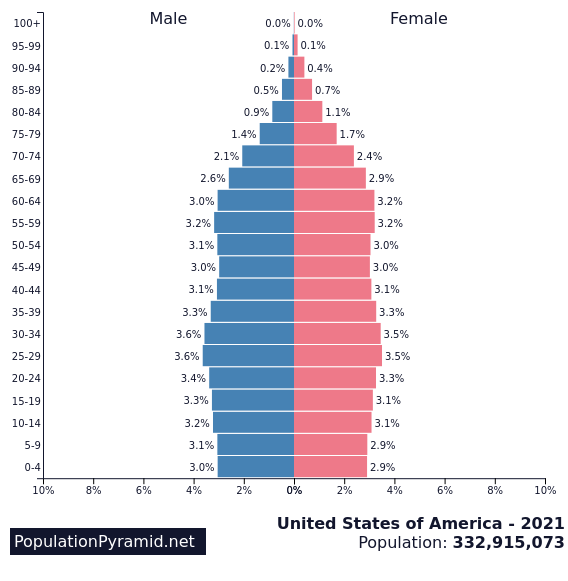
\includegraphics[width=7.25cm]{images/population_data/USA.png}}
	\qquad
	\subfloat[]{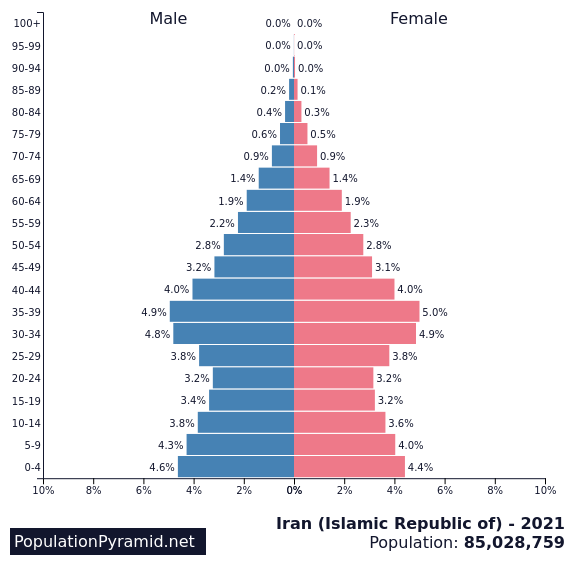
\includegraphics[width=7.25cm]{images/population_data/iran.png}}
	\caption[عنوان شکل در فهرست اشکال]
	{مقایسه هرم جمعیتی دو کشور (الف) ایران و (ب) آمریکا }
	\label{fig:intro:populationpyramid}
\end{figure} 

این یک متن نمونه است...این یک متن نمونه است...این یک متن نمونه است...این یک متن نمونه است...این یک متن نمونه است... این یک متن نمونه است...این یک متن نمونه است...این یک متن نمونه است...این یک متن نمونه است...این یک متن نمونه است...این یک متن نمونه است...این یک متن نمونه است...این یک متن نمونه است...این یک متن نمونه است... 
اینگونه رفرنس بدهید \cite{karimi2020soft, mohammadimohammadabadi}. 



% !TeX spellcheck = en_US
% Chapter 2
\chapter{مرور}\label{chap:review}

\section{بخش اول}\label{chap:brain}

این یک متن نمونه است...این یک متن نمونه است...این یک متن نمونه است...این یک متن نمونه است...این یک متن نمونه است... این یک متن نمونه است...این یک متن نمونه است...
برای بیان اکرونیم یک کلمه مانند  \gls{LASSO}، به این صورت عمل کنید.
   \gls{ML}
   یا 
   \gls{DL}
   یا
   \gls{FN}
   یا 
   \gls{TN}
   یا
   \gls{LSTM}
   یا 
   \gls{SGL}
   یا
   \gls{TP}
   یا 
   \gls{FP}
   یا
\subsection{زیربخش \gls*{1st}}\label{sec:brain:sub_brain}
این یک متن نمونه است که به سه مرحله \gls{1st}،
 \gls{2nd} و \gls{3rd} تقسیم می‌شود. 
 
 برای معادل جمع فارسی در دیکشنری اینطور فراخوان کنید: \glspl{2nd}
\begin{itemize}
	\item
	\gls{1st}: 
	این یک آیتم نمونه است...
		\item 
	\gls{2nd}: 
	این یک آیتم نمونه است...
	\item 
	\gls{3rd}: 
	این یک آیتم نمونه است...
\end{itemize}

\subsection{زیربخش دوم}\label{sec:brain:second_sub}
این یک متن نمونه است...


\paragraph{پاراگراف نمونه \gls*{1st}}
این یک متن نمونه است...
\paragraph{پاراگراف نمونه \gls*{2nd}}
این یک متن نمونه است...

\section{معرفی \gls*{dataset}}\label{sec:dataset}
این بخش نمونه است...

\begin{enumerate}
	
\item\textbf{فاز اول یا \lr{English-1}:} 
این یک متن نمونه است.
\begin{itemize}
	\item 
	این یک آیتم نمونه است...
	\item 
	این یک آیتم نمونه است...
	\item 
	این یک آیتم نمونه است...
\end{itemize}

این یک متن نمونه است...

\item\textbf{فاز دوم یا \lr{English-2}:} 
این یک متن نمونه است...

\item\textbf{فاز سوم یا \lr{English-3}:} 
این یک متن نمونه است...
\end{enumerate}

برای کامنت کردن بخشی از پروژه بدون حذف آن، از این دستور استفاده کنید.
\begin{comment}
برای کامنت کردن بخشی از پروژه بدون حذف آن، از این دستور استفاده کنید.
\end{comment}

برای درج جدول \ref{tab:my_table1} و رفرنس‌دهی از این کد استفاده کنید.

\begin{table}[t!]
	\centering
	\caption{جدول نمونه افقی}
	\label{tab:my_table1}
	\begin{tabular}{rccccc}
		\toprule			
		$\text{گروه}$ && $\text{فارسی (English)}$ & $\text{فارسی English}$ & $\text{فارسی English}$ & $\text{فارسی English}$ \\
		\midrule
		\rl{جنسیت}&(\rl{مرد - زن})	
		& $10 - 20$ & $10 - 20$ & $10 - 20$ & $10 - 20$
		\\
		\bottomrule
	\end{tabular}
\end{table}

برای درج جدول عمودی \ref{tab:my_table2} و رفرنس‌دهی از این کد استفاده کنید.
\begin{sidewaystable}
	\begin{threeparttable}
		\caption{جدول نمونه عمودی}
		\label{tab:my_table2}
		\setlength\tabcolsep{0pt} % make LaTeX figure out intercolumn spacing
		
		\begin{tabular*}{\columnwidth}{@{\extracolsep{\fill}} cccccccccc}
			\toprule			
			$\text{گروه}$ & 
			$\myfrac{\text{جنسیت}}{\text{مرد - زن}}$ & 
			$\myfrac{\text{فارسی}}{\text{\lr{mean$\pm $std}}}$ & 
			$\myfrac{\text{ٍenglish}}{\text{\lr{mean$\pm $std}}}$ & 
			$\myfrac{\text{فارسی}}{\text{\lr{mean$\pm $std}}}$ & 
			$\myfrac{\text{\lr{english}}}{\text{\lr{mean$\pm $std}}}$ & 
			$\myfrac{\text{\lr{ٍenglish}}}{\text{\lr{mean$\pm $std}}}$ & 
			$\myfrac{\text{ٍenglish}}{\text{\lr{mean$\pm $std}}}$ & 
			$\myfrac{\text{\lr{ٍenglish}}}{\text{\lr{mean$\pm $std}}}$ & 
			$\myfrac{\text{\lr{RAVALT-PF}}}{\text{\lr{mean$\pm $std}}}$ \\
			\midrule
			فارسی AD & $189 / 153$ & $75.0 \pm 7.8$ & $4.39 \pm 1.67$ & $15.2 \pm 3.0$ & $19.6 \pm 6.7$ & $29.9 \pm 8.1$ & $23.2 \pm 2$ & $22.8 \pm 7.6$ & $89.0 \pm 21.2$ 
			\\
			\bottomrule
		\end{tabular*}
	\end{threeparttable}
\end{sidewaystable}

\section{فرمول}\label{sec:formula}
بنابراین برای هر نقطه $X$ از تصویر سه بعدی دریافتی، رابطه
\begin{align} \label{eq:n3-main}
	v(X) = u(X) f(X) + n(X)
\end{align}
برقرار است که $v$ سیگنال اندازه‌گیری شده، $u$ سیگنال مورد انتظار بدون اثر \gls{bias} میدان و $f$ یک سیگنال با تغییرات آرام و نماینده \gls{bias} میدان است.
روابط تبدیل فوریه تابع $f(t)$ و معکوس آن به بیان شده در روابط \ref{eq:fourier} و \ref{eq:afourier}  هستند.
\begin{align}\label{eq:fourier}
\mathcal{F}(f(t))= F(w)=\sum_{k=0}^{N-1}f_k e^{-i\frac{2\pi}{N}kn}
\end{align}
\begin{align}\label{eq:afourier}
f_k= F(w)=\frac{1}{N}\sum_{n=0}^{N-1}\mathcal{F}_n e^{-i\frac{2\pi}{N}kn}
\end{align}


% Chapter 4
\chapter{فرمول}
\label{chap:propml}

نمونه‌های فرمول چندخطی:
\begin{align}
Loss(t,y(x)) & = \{y(x)-t\}^2 \nonumber\\ 
& = \{y(x)- \mathbb{E}_{t}[t|x] + \mathbb{E}_{t}[t|x] -t\}^2 \nonumber \\ 
& = \{y(x)- \mathbb{E}_{t}[t|x]\}^2 + 2\{y(x)- \mathbb{E}_{t}[t|x]\}\{\mathbb{E}_{t}[t|x] - t\} + 
\{\mathbb{E}_{t}[t|x] -t\}^2 
\end{align}
برای رفرنس دهی به رابطه \eqref{eq:biasvar_bias_var} اینگونه عمل کنید.
\begin{multline}
\label{eq:biasvar_bias_var}
\mathbb{E}_\mathcal{D} [\{y(x;\mathcal{D})-\mathbb{E}_{t}[t|x]\}^2] \\
=\{\mathbb{E}_\mathcal{D}[y(x;\mathcal{D})]-\mathbb{E}_{t}[t|x]\}^2 + 
\mathbb{E}_\mathcal{D}[\{y(x;\mathcal{D})-\mathbb{E}_\mathcal{D}[y(x;\mathcal{D})]\}^2] 
\end{multline}
برای نوشتن فرمول چندبخشی اینگونه عمل کنید.
\begin{subequations}
	\begin{equation}
	\text{\gls{variance}} = \int{\mathbb{E}_\mathcal{D}[\{y(x;\mathcal{D})-\mathbb{E}_\mathcal{D}[y(x;\mathcal{D})]\}^2]p(x)dx}
	\end{equation}
	\begin{equation}
	\text{\gls{bias}} = \int{\{\mathbb{E}_\mathcal{D}[y(x;\mathcal{D})]-\mathbb{E}_{t}[t|x]\}^2p(x)dx}
	\end{equation}
	\begin{equation}
	\text{\gls{noise}} = \int{\{\mathbb{E}_{t}[t|x] -t\}^2p(x)dx}
	\end{equation}
\end{subequations}
دیگر نمونه فرمول ها:
\begin{equation*}
G=
\begin{bmatrix}
G_{11}&G_{12}\\G_{21}&G_{22}
\end{bmatrix} 
\end{equation*}

\begin{equation*}
\left\{\begin{array}{l}
z=G_{11}w+G_{12}u\\
y=G_{21}w+G_{22}u
\end{array}\right. 
\end{equation*}

برای رسم دیاگرام به صورت مستقیم، اینگونه عمل کنید.
\setlength{\unitlength}{1cm}
\begin{figure}[t]
	\centering
	\lr{
		\begin{picture}(10.5,2.3)(0,0)
		\put(0,1.5){\vector(1,0){1.35}}
		\put(0.675,1.7){\makebox(0,0)[b]{$r(t)$}}
		\put(1.2,1.7){\makebox(0,0){$ \scriptstyle + $}}
		\put(1.5,1.5){\circle{0.3}}
		\put(1.65,1.5){\vector(1,0){1.35}}
		\put(2.325,1.7){\makebox(0,0)[b]{$e(t)$}}
		\put(3,1){\framebox(1.5,1){$K(t) $}}
		\put(4.5,1.5){\vector(1,0){1.5}}
		\put(5.25,1.7){\makebox(0,0)[b]{$u(t)$ }}
		\put(6,1){\framebox(1.5,1){$G(s)$}}
		\put(7.5,1.5){\line(1,0){1.5}}
		\put(9,1.5){\circle*{0.08}}
		\put(9,1.5){\vector(1,0){1.5}}
		\put(9.75,1.7){\makebox(0,0)[b]{$y(t)$}}
		\put(9,1.5){\line(0,-1){1.5}}
		\put(9,0){\line(-1,0){7.5}}
		\put(1.5,0){\vector(0,1){1.35}}
		\put(1.3,1.2){\makebox(0,0){$ \scriptstyle - $}}
		\end{picture}
	}
	\caption{یک سیستم زمان‌پیوسته}
	\label{fig:sample}
\end{figure} 



% Chapter 5
\chapter{نتیجه‌گیری و پیشنهادها}

\section{نتیجه‌گیری}
این یک متن نمونه است...این یک متن نمونه است...این یک متن نمونه است...این یک متن نمونه است...این یک متن نمونه است... این یک متن نمونه است...این یک متن نمونه است...این یک متن نمونه است...این یک متن نمونه است...این یک متن نمونه است...این یک متن نمونه است...این یک متن نمونه است... این یک متن نمونه است...این یک متن نمونه است...

\section{پیشنهادها}
این یک متن نمونه است...این یک متن نمونه است...این یک متن نمونه است...این یک متن نمونه است...این یک متن نمونه است... این یک متن نمونه است...این یک متن نمونه است...این یک متن نمونه است...این یک متن نمونه است...این یک متن نمونه است...این یک متن نمونه است...این یک متن نمونه است... این یک متن نمونه است...این یک متن نمونه است...
ه





%% Appendices
%\appendix
%\include{app1}

%print dict and acn pages
\printglossary

% ‎References‎
‎\renewcommand{\bibname}{مراجع}‎
‎\addcontentsline{toc}{section}{مراجع}‎

‎%%You may use IEEE transactions style‎
%\bibliographystyle{ieeetr-fa}‎
‎\bibliographystyle{ModifiedIEEEtranFa}‎
%‎\bibliographystyle{plain-fa}‎ %added by ehsan
‎%You may use IEEE abbreviation along with the name of your bitex database‎.
‎\bibliography{my_ref}

\addcontentsline{toc}{section}{چکیده انگلیسی}
\thispagestyle{empty}

\begin{latin}
\begin{center}

{\huge Title of thesis comes here}

\vspace{1cm}

{\LARGE{Bahram Bahrami Bahramabadi}}

\vspace{0.2cm}

{\small example@example.ir}

\vspace{0.5cm}

Feb 19, 2022

\vspace{0.5cm}

Department of Electrical and Computer Engineering

\vspace{0.2cm}

Isfahan University of Technology, Isfahan 84156-83111, Iran

\vspace{0.2cm}

Degree: M.Sc. \hspace*{3cm} Language: Farsi

\vspace{1cm}

{\small\textbf{Supervisor: Prof. Mohammad Mohammadi Mohammadabadi (example@example.ir)}}
\end{center}
~\vfill


\noindent\textbf{Abstract}

\begin{small}
\baselineskip=0.6cm

Lorem ipsum, or lipsum as it is sometimes known, is dummy text used in laying out print, graphic or web designs. Lorem ipsum, or lipsum as it is sometimes known, is dummy text used in laying out print, graphic or web designs. Lorem ipsum, or lipsum as it is sometimes known, is dummy text used in laying out print, graphic or web designs. Lorem ipsum, or lipsum as it is sometimes known, is dummy text used in laying out print, graphic or web designs. 

\end{small}

\vspace{0.5 cm}

\noindent \textbf{Key Words}: Example, Example, Example, Example

\end{latin}
%********************************
% Page before last: English Signatures
%********************************
\thispagestyle{empty}
\newgeometry{left=3cm,right=3cm,top=2cm}
\begin{latin}
\begin{center}

\includegraphics[height=3cm]{images/iut_logo.png}
\vspace{0.4cm}

{\large\textbf{Isfahan University of Technology}}\\

\vspace{0.4cm}
Department of Electrical and Computer Engineering

\vspace{2.5cm}

{\huge Thesis title comes here}

\vspace{1.5cm}

{\large
	A Thesis
	
	\vspace{.3cm}
	
	Submitted in partial fulfillment of the requirements
	
	\vspace{.3cm}
	
	for the degree of Master of Science
}

	\vspace{1.5cm}

{\Large
	\textbf{by}
	
	\vspace{.3cm}
	
	\textbf{Bahram Bahrami Bahramabadi}
}
\end{center}

\vfill

Evaluated and Approved by the Thesis Committee, on Jan 01, 2022
\vspace{0.5cm}

\begin{enumerate}
\item Mohammad Mohammadi Mohammadabadi, Prof. (Supervisor)
\vspace{0.5cm}

\item Mohammad Mohammadi Mohammadabadi, Assoc. Prof. (Advisor)
\vspace{0.5cm}

\item Mohammad Mohammadi Mohammadabadi, Prof. (Examiner)
\vspace{0.5cm}

\item Mohammad Mohammadi Mohammadabadi, Assist. Prof (Examiner)
\vspace{0.5cm}

\end{enumerate}

Mohammad Mohammadi Mohammadabadi, Department Graduate Coordinator

\pagebreak
\end{latin}

%***************************
% last page: Blank
%***************************
\thispagestyle{empty}
\mbox{}

% It's finally over. Wasn't that hard, was it?
\end{document}